\documentclass{scrartcl}
\usepackage{graphicx}
\usepackage[utf8]{inputenc}
\usepackage[english]{babel}
\usepackage{amsthm}
\usepackage{amsmath}
\usepackage{amssymb}
\usepackage[hyphens]{url}
\usepackage{listings}
\usepackage{syntax}
\usepackage{color}
%\usepackage{algorithm}
\usepackage{algpseudocode}
\usepackage{subcaption}
\usepackage{placeins}
\usepackage{booktabs}
\usepackage[page]{appendix}
\usepackage{enumerate}
\usepackage{syntax}
\usepackage{proof}
\usepackage{stmaryrd}
\usepackage{biblatex}

\newcommand{\code}[1]{\texttt{#1}}
\newcommand{\mcode}[1]{\mathbf{#1}}
\newcommand{\while}{While}
\newcommand{\den}[1]{\llbracket #1 \rrbracket}

\newcommand{\infname}[1]{\text{\textsc{#1}}}
\newcommand{\whil}{\mcode{while}\ b\ \mcode{do}\ S}

\newtheorem{lem}{Lemma}
\newtheorem{col}{Corollary}

\addbibresource{biblio.bib}

\title{Compiler for the Simple Programming Language}
\author{Andreas Vinter-Hviid \and Ronan Guillaume}
\date{June 15, 2017}

\begin{document}
\maketitle

\tableofcontents

\section{Introduction}
This report describes our implementation of a compiler for the Simple
Programming Language (SPL).

We have chosen to implement the compiler in Haskell. This is mainly
due to the fact that it is a high level language with
support for algebraic data types and pattern matching
which makes working with syntax trees easier. There are more languages
which lives up to these criteria. Haskell has been chosen among
these primarily because of familiarity to us, and the fact that it is
a widely used language with good documentation and tooling.

We have approximately 1800 lines of code in our compiler plus 126 lines
of test code and an additional 580 lines of test data (that is SPL
programs we are using for the tests).
\section{Parser and Scanner}
Parsing is done using parser combinators, which for the vast 
majority of the given grammar allows us to translate the BNF
grammar rules more or less directly to
Haskell code.

Scanning is also done with parser combinators, but finding longest
matches requires a little bit of cleverness. This involves using a
predicative version of the alternative combinator, which only tries
the second alternative if the first does not work and ordering all
operator and symbol tokens by length. This will not work for 
identifiers or keywords since the first do not have fixed length and
we don't want prefixes of identifiers which look like keywords to be
interpreted as keywords. Instead we simply use parser combinators
to parse any type of words (using the predicative alternative to 
only get the longest) and then afterwards we check if the word matches
a keyword or if it is an identifier.

\subsection{Parser combinators}

For the parser and scanner we have implemented our own parser combinator
library. The basic principles are those presented in class, but error
handling capabilities have been added, which turns out to complicate
things quite a bit.

The type of a parser is as follows:
\begin{lstlisting}
type ParseSuccesses t a = NonEmpty (a, [(Integer, t)])
type ParseError t = ((Set.Set t), Maybe (Integer, t))

data ParseResult t a = 
      Success (ParseSuccesses t a)
    | Error (ParseError t)
    | Uncertain (ParseError t) (ParseSuccesses t a) deriving (Show)

data Parser t a = Parser ([(Integer, t)] -> ParseResult t a)
\end{lstlisting}
Ignoring the \lstinline{Uncertain} case for a moment,
A parser is a function from a list of Integer, token pairs to either
an error or a non empty list of results and remaining output.
Normally it would be possible to use an empty list as error indicator,
but since we want additional information with the error this is not
possible. The reason for pairing each token with an integer is so that
we get an ordering on tokens. The idea is to pair the tokens with 
increasing numbers, so that we can tell which of two tokens is furthest
ahead in the input.

This is important because we want to always report the error that
happened the furthest ahead. Consider for example 
syntax errors in function definitions.
They make the function definition actually invalid,
and instead of complaining about the specific syntax error inside the
function, the parser will conclude that there are no more function
definitions and complain that the attempt at defining a function
shows up when it was expecting the end of the file. This is not
desirable, we want an error about what is wrong inside the function
definition.

\begin{figure}
\centering
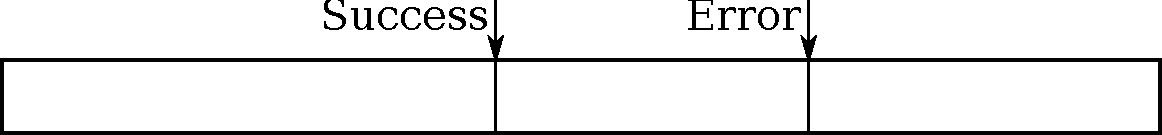
\includegraphics[width=0.75\textwidth]{drawing}
\caption{Illustration of \lstinline{Uncertain}}
\label{fig:uncertain}
\end{figure}

More generally, we can have a situation like the one depicted in 
figure \ref{fig:uncertain}. We have a successful parse and an error
further ahead. We do not want to throw the error away, because it is
not guaranteed that continuing parsing from the success gets us further
than the error. There are three cases
\begin{enumerate}
\item A list of successful parses with no errors further ahead
\item A list of successful parses with errors further ahead
\item No success.
\end{enumerate}
These correspond to the \lstinline{Success}, \lstinline{Uncertain}, and 
\lstinline{Error} constructors respectively. When combining two parses
care must be taken to figure out what type of result the combination
of two things becomes.

Note that for parsers which requires to match the end of file, an
\lstinline{Uncertain} result will eventually turn in to either an
error or a success. Either there will be a successful result of
parsing all the input in which case there can not be errors further
ahead, or all potential successes (including the uncertain ones) will
turn into errors by continued parsing.

\subsection{Precedence and associativity}

With parser combinators many aspects of the BNF grammar can be
almost directly copied to create the parser. The problems of 
precedence and associativity however requires some care. I will start
by discussing precedence.

Getting precedence to work is a question of making
sure that the parse tree which is used to recognize the input is
a certain one. That is to unambiguiate the grammar. The possible
binary operators are divided into $n$ precedence levels 
from $0$ to $n-1$. The
$\text{op2}_n$ rule recognizes operators on the $n$th level. Table
\ref{tab:precedence} shows the precedence levels in our implementation.

\begin{table}
\centering
\begin{tabular}{| c | l | }
\hline
0 & $==$, $\neq$ \\
\hline
1 & $<$, $>$, $\leq$, $\geq$ \\
\hline
2 & $:$ \\
\hline
3 & $+$, $-$, $||$ \\
\hline
4 & $*$, $/$, $\%$, $\&\&$ \\
\hline
\end{tabular}
\caption{Precedence levels for the operators in SPL. As it can be seen
 in our case $n=4$, but this is easily extended to any number of
levels}
\label{tab:precedence}
\end{table}

Expressions are divided into $n + 1$ levels. On the $i$th level are 
expressions which are a number of expressions combined by a level
$i$ binary operator. The first of these expressions is a level
$i+1$ expression
and the remaining are level $i$. The $n$th level contains all 
expressions which are not applications of binary operators.
The only one of these which is non trivial is the application of a
unary operator,
since it contains a sub expression, and we have to decide on a
level for this sub expression. Making this a level $n$ expression
causes unary operators to have highest precedence, which is the
desired effect.
That is for $0 \leq i < n$ the grammar looks as
\begin{align*}
\text{exp}_i ::=&\ \text{exp}'_i\ [ \text{op2}_i\ \text{exp}_i ] \\
\text{exp}'_i ::=&\ \text{exp}_{i+1} 
\end{align*}
And for $n$ we have defined:
\begin{align*}
\text{exp}'_{n} ::=&\ \ldots \\
    | &\ \text{op1}\ \text{exp}'_{n} \\
    | &\ \ldots
\end{align*}
Here the dots represent all the non operator expression types.

Associativity is handled by taking the list (a list is a type of tree)
produced by the expression parser for a given level and do either
a left fold or a right fold over it to translate it into the final
AST representation. That is, for each precedence level there is a
fixed associativity. This is left for all of the levels except for
level 2 where it is right. Having two operators with different
associativity on the same precedence level does not make sense.

\section{Type inference}
The typing system supports let-polymorphism and full inference of types.
It is based on Hindley-Milner type inference as presented in the
lectures. We will not repeat that here, but only explain how we 
concertized the idea to work in our compiler. Adapting the theory
to concrete code was more challenging for the type inference than
in any other parts of the compiler.
Therefore this section will
be relatively heavy in implementation details.

\subsection{Substitutions}

In the type checking algorithm the concept of a substitution will
play an important role. There will be many type-related objects including
type, type contexts, and type schemes to which we can apply 
substitutions. Furthermore substitutions can be composed and as we
will see defining the concept of applying a substitution to various
Haskell specific constructs can make the code a bit nicer. This
section will be about how we concretely implemented substitutions.

A substitution is just a list of pairs mapping a type variable name
to a type.
\begin{lstlisting}
data Substitution = Substitution [(TVarId, Type)]
\end{lstlisting}
Substitutions form a monoid under composition
\begin{lstlisting}
instance Monoid Substitution where
    mempty = Substitution []
    mappend (Substitution s1) s2'@(Substitution s2) = Substitution  
        (fmap (\(id,t) -> (id, subst s2' t)) s1 ++ s2)
\end{lstlisting}
Basically applying the second substitution to the first one, and then
appending the second one to the result.

In order to overload the concept of substitution so a substitution
can be applied to many things, we introduce a type class
\begin{lstlisting}
class Substable a where
    subst :: Substitution -> a -> a
\end{lstlisting}
This class is instantiated for types, type contexts
in the obvious ways. It is also instantiated for substitutions in which
case the subst function is just mappend.

In the unification and type inference algorithm, there are many
cases of having to perform a substitution on each argument to a
function which returns a substitution and then compose the
first substitution with the result. For example in this case from
the unification algorithm:
\[ \mathcal{U}((\sigma_1, \sigma_2),(\tau_1, \tau_2)) = \
   \mathcal{U}(\sigma_2^*,\tau_2^*) \circ * \text{, where }
   * = \mathcal{U}(\sigma_1, \tau_2) \]
To make this a bit prettier we define the notion of substitution on
a function from substitutable things to substitutable things:
\begin{lstlisting}
instance (Substable a, Substable b) => Substable (a -> b) where
    subst s f = \a -> subst s (f (subst s a))
\end{lstlisting}
With this in place the previously mentioned rule of the unification
algorithm can be written as
\[ \mathcal{U}((\sigma_1, \sigma_2),(\tau_1, \tau_2)) = \
   \mathcal{U}(\sigma_2,\tau_2)^* \text{, where }
   * = \mathcal{U}(\sigma_1, \tau_2) \]

The actual unification algorithm is exactly as it was presented in
class. It is possible for unification to fail, so the return type
is not actually just a substitution, but an \lstinline{Either}.
Therefore one can also substitute into an either provided that the
type of the right type is substitutable. Similarity in the actual
interference algorithm we are working in a more complicated state
monad which contains, among other things, a typing context.
This monad has also been made
substitutable with the extra detail that the substitution also gets
applied to this context.

\subsection{Typing rules}
In the case of expressions the algorithm presented can very directly
be applied. For statements some adaptation is needed. The main
things to take into consideration are (2 and 3 are related)
\begin{enumerate}
\item The value restriction
\item Checking the type of a function declaration
\item Making sure that a function returns
\end{enumerate}
Addressing the first point: Generally declarations are treated as let
bindings. However if we are binding a mutable value to a name, as in
a variable definition, the polymorphism needs to be restricted for 
the type system to be safe. This is done by instead of letting all
unbound type variables be universally quantified, letting none of them
be. This is known as the value restriction. Functions are then the
only things with truly polymorphic types.

Regarding the second and third point: Figuring out the type of a 
function, in particular the return type, is more complicated in a
language with statements than in one with only expressions. We 
ignore the types of all statements except for return statements or
statements that contain a return in them. The following restrictions
are then made
\begin{enumerate}
\item All returns must be of unifiable types
\item All functions must return something
\end{enumerate}
The most general unifier of all returns is then the return type of
a function. Checking 1 is a matter of trying to unify all return
types. Checking 2 is a bit more involved.

We use the following method, which involves keeping a stack of booleans
around. This goes into the state we are already carrying around by
in a state monad.
\begin{itemize}
\item Initially the stack is \lstinline{[False]}.
\item When a return is encountered set the top element to \lstinline{True}.
\item When entering a branch of a control structure push False on the stack.
\item When leaving \emph{the last} branch of a control structure pop the number of branches elements from the stack. Then:
\begin{itemize}
  \item let $x$ be the conjunction of the popped elements.
  \item If one of the branches is guaranteed to be executed set the top element to be the disjunction of itself and $x$.
\end{itemize}
\end{itemize}
If the stack contains exactly the single element false when
reaching the end of a statement list, then a return is missing.
Instead of rejecting the program we insert an implicit void return.
If this return conflicts with another return in the function definition,
one inside an if statement for instance, it will be a type error.

This approach makes sure to not add returns inside control structures
and in the case of an if/else with a return in both branches it 
detects that a return is guaranteed.


\subsection{Missing features}
\label{sec:type:missing}
We have not been able to make type annotations work. They can be
written and are accepted by the parser, but during type inference
they are completely ignored.

During development of the typing system we were mainly concerned with
checking that a program is typeable. We made the mistake of not 
actually storing the inferred type information anywhere. This type
information can be very valuable in later stages of the compiler, so
we should have saved it.

\section{Code generation}

Code generation is handled by recursively traversing the AST, generating
a list of instructions at each node by pasting together the code
generated by the children and adding relevant extra instructions.

During this traversal some state is kept using a state monad. In
particular we keep track of an integer used to generate unique label
names, and the current variable context, i.e. a map
from variable names to integers representing where they can be found
relative to the base pointer(MP) of the current stack frame.

In addition the function for generating code for an expression node
takes a boolean argument, which will be expanded upon in section
\ref{sec:gc}, and the function for generating code for a statement
node takes a string denoting the label to jump to in the case of a 
return statement.

\subsection{Stack layout}
One of the key design decisions in code generation is the stack
layout. The SSM has nice instructions for dealing with call stacks
which suggest a certain design. We have mainly used this, but in
order for garbage collection to work we have some extra constraints 
which needs to be handled which complicates the stack layout a little
bit.

\begin{enumerate}
\item At runtime we have to know how many local variables 
including arguments are 
associated with a frame, and where they are.
\item A local can only contain a reference to a heap object if that
heap object is actually alive.
\end{enumerate}
\begin{table}
\centering
\begin{tabular}{l | c |}
  & arg $n$ \\
\cline{2-2}
  & ... \\
\cline{2-2}
  & arg 2 \\
\cline{2-2}
  & arg 1 \\
\cline{2-2}
  & ret. addr.  \\
\cline{2-2}
MP& old MP \\
\cline{2-2}
  & $m+n$ \\
\cline{2-2}
  & local $m$ = 0 \\
\cline{2-2}
  & ... \\
\cline{2-2}
  & local 2 = 0\\
\cline{2-2}
  & local 1 = 0 \\
\cline{2-2}
  & copy of arg 1 \\
\cline{2-2}
  & copy of arg 2 \\
\cline{2-2}
  & ... \\
\cline{2-2}
SP& copy of arg $n$ 
\end{tabular}
\caption{Stack layout after prologue of function has been executed}
\label{tab:stackframe}
\end{table}
Table \ref{tab:stackframe} shows what a stack frame looks like right
after the function prologue has been run. The main differences from
what a stack frame created by a normal \lstinline{bsr funcion} followed
by a \lstinline{link m} is the following:
\begin{enumerate}
\item An extra field containing the total number of locals ($m+n$)
 has been added right after the MP.
\item All arguments have been copied into local variable space.
\item All newly created local variables that are not arguments have
 been zeroed.
\end{enumerate}
The first two points makes sure that the garbage collector can easily
find and traverse through all variables associated with a frame.
The third point makes sure that a local will not accidentally contain
a pointer to some heap structure which is not actually in use.

In the actual body of the function arguments are always obtained
through the copy in local variable space. The arguments supplied by
the caller are not used after they have been copied initially.

\subsection{Pairs and lists}

All basic types, booleans, integers (and void)  are represented by a
single word and passed around to functions as values.

For pairs and lists this will not work, not only do they not fit into
a single word, because they can be nested they can be of arbitrary 
size. Therefore all pairs and lists are allocated on the heap. On
the stack and when passed to functions they are represented by a
reference to their heap object. This reference is also passed by value.

Discussion of the exact structure of a heap object is deferred to
section \ref{sec:gc:heap}. For now we just assume the existence of 
a subroutine (not directly accessibly by the programmer) which takes
two words, stores them in a new heap object, and returns a reference
to this new object.

Every time the syntactical form \lstinline{(X, Y)} is encountered a
new pair is allocated with \lstinline{X} and \lstinline{Y} as data.

Lists are linked lists. This fits the syntax. Creating array semantics
for cons/nil hd/tl style syntax would be cumbersome, and probably end
up with a lot of reallocations and inefficient code in general. This
means that a list can either be nil, which is represented by the value
0 or it can be a cons cell containing some data and a next pointer.
Cons cells are treated similarity to pairs.

\subsection{Missing features}

The code generation of our compiler has some missing features. The
two main ones are support for global variables and the overloaded print
function. As mentioned in section \ref{sec:type:missing} due to the
way we designed the type checker we do not actually have type information
at later stages. This is problem when trying to implement overloaded
functions.

In addition labels in the assembly code are not handled super rigorously.
It might be possible to write code that produces assembler with two
identical labels at different places in the code. Also a main function
is required, but that it actually exists is not checked. A branch
instruction to a main label is just inserted after the initial setup
code.

\section{Garbage collection}
\label{sec:gc}
As our extension we have chosen to implement garbage collection, so that
memory can be reclaimed without the programmer having to manually free
it. We have implemented a copying garbage collector. It works by splitting 
the heap space into two equally sized parts. Only one of the parts is 
in use at a time. When there is no more space in that part a collection
is initiated. The collection makes the other part of the heap the 
currently active one and then reallocates all heap object from the old
part which are still in use. All references pointing to copied(reallocated)
objects needs to be updated. This removes all heap object to which no
references exists, while completely avoiding fragmentation. The cost is
that the user can only use half of the available memory space 

\subsection{Heap object layout}
\label{sec:gc:heap}
All heap objects take up 4 words of memory. Only 3 of these are used,
but we need an even number to keep alignment. The layout is shown
in table \ref{tab:heapobj}. Two words are used for the data. Head and 
tail or first and second depending on whether it is a list or a 
pair. In theory it would be
possible to reduce the size to 2 words since we only need the forwarding
pointer when the data does no longer matter.

\begin{table}
\centering
\begin{tabular}{| c |}
\hline
unused \\
\hline
forwarding pointer \\
\hline
data \\
\hline
data \\
\hline
\end{tabular}
\caption{Heap object layout}
\label{tab:heapobj}
\end{table}

When allocating a new object, we need to set the forwarding pointer
such that it is guaranteed to not point the currently inactive
region of heap memory. In our implementation it points to the beginning
of the heap object, only because that was convenient. It could just
as well have replicated one of the data fields, or been set to a consant
even number.

When allocating it is also checked if there is enough heap space.
If not a collection is initiated.

\subsection{Tagging}

The algorithm, which will be elaborated in more detail later, 
 depends on being able to discern between references and
values at runtime. Since the heap pointer starts at an even address, 
all heap objects have size 4, and references point to the end of heap
objects, every reference will be an odd number. We make sure to multiply
all values by two before storing them to a memory location (and 
dividing them by two again before doing computation with them on the
stack). This process we refer to as tagging (and untagging). In the
case of references tagging and untagging them is simply a no op(In
addition tagging and untagging the value 0 is also a no op, this is 
important because lists are always either references or 0 in the case
of nil).
This provides a method of discerning values from references, namely
parity. 

Actually realizing this is not completely trivial. Untagging is always
quite easy, because we can use the tag to determine how to untag
\footnote{However we don't actually even have to do this, it turns
out we can completely determine if we are untagging a reference or a 
value at runtime. This will be elaborated later}. Tagging is the more
difficult process because it is not always trivial to see if we are
dealing with references or values. The process of
tagging happens in assignment statements
\begin{lstlisting}
a = X;
\end{lstlisting}
where \lstinline{X} is any kind of expression. It is tempting to 
let all expression code deal exclusively in untagged values (by 
immediately untagging any value loaded from memory and never tagging
anything) and then
tagging right before assignment, in the statement generating code.
This works in most cases because we know whether the result of an 
expression is a reference or a value. However, consider the case where
\lstinline{X} is just a variable. In this case it is not known whether
we are dealing with a reference or a value. To find this out type
information would be needed, but as explained in section \ref{sec:type:missing}
it is not available and making it so seems like a lot of work.

Stepping a bit back, actually storing one variable into another is just
moving a tagged value from one place to another. We should not actually
have to do anything to it, and therefore we should be able to perform
this operation without type information. This is indeed possible, but
it requires the code generation for expressions to be able to work 
with tagged values.

The way we solve this is by having the expression code generation
function taking an argument which specifies whether it should deliver
a tagged or an untagged value on the stack. Pushing conversions down
like this, which allows us to completely avoid them if they are not
needed, turns out to work remarkably well even without type
information. Maybe it should not be surprising that this is 
possible since if we are able to generate code without type information,
we should also be able to determine if something is a value or a 
reference without it. How else could we generate the code in the
first place?

There is even a trick we can use, exploiting that untagging a reference
is a no op. If we generate code for an expression and we know that it
will result in a reference, we can ask for a tagged value even if we
need an untagged one. Applying this everywhere it turns out that we
can avoid every single situation where untagging a reference would
otherwise be needed. This means that the untagging code simply becomes
division by 2. There is no need to check if we are trying to untag a
reference, because we never are.

\subsection{Cheney's algorithm}

In this section the garbage collection algorithm itself is described
in more detail. Fundamentally it is Cheney's algorithm \cite{cheney}.

They key part is the \emph{forward} operation. The rest of the algorithm
is just about applying this to the right things in the right order.
The forward operation takes a pointer, makes sure the object pointed
to has been reallocated on the new active part of the heap, and then
returns the new location. It works in three steps as described below.

\begin{enumerate}
\item If the input is not a pointer, or already points to new part of
 heap, return the input directly.
\item If the forwarding pointer of the object pointed to by the input
 points to the new part of the memory, return the forwarding pointer.
\item Otherwise reallocate the data, then set the forwarding pointer of
 the old object to the new location. Return the pointer to the new location.
\end{enumerate}

Note that this procedure is not recursive. If a heap object itself
contains pointers, just forwarding it is not enough. We explicitly
want to move all the active objects to the new heap in a breath first
way. This greatly simplifies updating all pointers.

Now for the actual algorithm. The first step is changing which half
of the memory space we use. In order to keep track of our memory three
values, all stored in registers are used. The first is the standard
heap pointer (R3/HP), which tells us where to next allocate memory.
Next the \emph{limit} of the current part of memory is held in R5.
Finally the \emph{other} value in R6 points to the beginning of the
part of memory not currently in use. Also recall that R7 holds to initial
value of MP, which is not a valid stack frame.

\begin{algorithmic}
\State $scan \gets \mathrm{R6}$ \Comment{R6 is other}
\State $\mathrm{R6} \gets \mathrm{R5} - size$ \Comment{R5 is limit}
\State $\mathrm{R5} \gets scan + size$
\State \Comment{Now the active part of the heap is changed, and $scan$ points
to beginning of newly activated part}
\State $base \gets [\mathrm{MP}]$
\While{$base \neq \mathrm{R7}$} \Comment{forward roots}
    \State $i \gets 2$
    \State $locals \gets [base + 1] + 2$
    \While{$i < locals$}
        \State $[base + 1] \gets \mathrm{forward}([base + 1])$
    \EndWhile
    \State $base \gets [base]$
\EndWhile
\While{$scan < \mathrm{HP}$} \Comment{forward rest by bfs}
    \State $[scan + 2] \gets \mathrm{forward}([scan + 2])$
    \State $[scan + 3] \gets \mathrm{forward}([scan + 3])$
    \State $scan \gets scan + 4$
\EndWhile
\end{algorithmic}
The first while loop forwards all pointers in local variables.
The next scan through the new heap and forwards all pointers
of newly allocated objects, until no more objects are being moved
to the new heap space.

This is all implemented in assembler and appended onto every program.

\section{Tests}

Throughout the development we have used various techniques for testing.
For the parser/scanner and type checker we have an automatic test
suite. For the parser/scanner we read in a number of programs, then
write you the result and read it in again. The we compare the two 
generated abstract syntax trees for equality.

For the type inference we have a number of type correct programs
which we read in and type check. Then make sure they are not rejected.
We also have a collection of type incorrect programs which we make
sure are rejected. In particular we test various features such as the
value restriction and return statements here.

The following program type checks, which shows that polymorphism works.
\begin{lstlisting}
id (x) {return x;}

test () {
    var a = id(4);
    var b = id(True);
    return;
}
\end{lstlisting}
The following program is rejected by the type checker. This is the
value restriction coming into play. Even though \lstinline{a} has
type \lstinline{[a]}, the type variable is not truly universally
quantified, and as soon as we assign \lstinline{True : []} to \lstinline{a}
the type is restricted to \lstinline{[Bool]}.
\begin{lstlisting}
main () {
    var a = [];
    a = True : [];
    a = 1 : [];
    return;
}
\end{lstlisting}

For the Code generation and garbage collection the testing is more
manual. We still have a collection of SPL programs which test various
features, but that they work is verified manually


The following program is for testing the garbage collector. It is meant
to be run with a heap size of only 16 words (times two).
The workings of the program is explained in the comments.
\begin{lstlisting}
g(x) {
    var y = 3 : x; //points to already refernced data
    var a = [];

    x = []; //Lose last direct reference to this memory
            //x is now only referenced through other heap objects

    a = 4 : []; //This causes GC for 16 word test heap.
}

main () {
    var x = 1 : 2 : []; //Create some data to not collect.
    var a = 0 : [];
    a = []; // Create some garbage to collect.
    g(x.tl);

    x = []; //Forget everything.
    x = 1 : []; // Cause GC again, to test on other heap.
}
\end{lstlisting}
When the first collection is initiated, the heap contains the list
\lstinline{x = 1 : 2 : []} which is alive reachable from \lstinline{main}s 
stack frame,
the list \lstinline{a = 0 : []} which is garbage, and the list 
\lstinline{y = 3 : 2 : []} in \lstinline{g}s stack frame sharing the
\lstinline{2 : []} part with \lstinline{x}.

That the collection works is verified by single stepping through the 
program and making sure everything works as intended. Especially for
the garbage collector this is cumbersome, but testing this kind of 
thing automatically would require a lot of debugging infrastructure.

\printbibliography


\end{document}
